\documentclass[12pt,fleqn]{article}\usepackage{../../common}
\begin{document}
Paralel Lojistik Regresyon, Eşle/İndirge

Lojistik regresyon kodunu eşle-indirge (map-reduce) üzerinden paralelize
etmek için literatüre [1-7] bakınca, genel yaklaşımın makinalara bölünen
veri parçaları üzerinde ayrı ayrı gradyan çıkışının (gradient aşçent)
işletilmesi ve sonuç $\theta$'ların son bir makinada ortalamasının alınması
olduğunu görürüz.

Daha önceki lojistik regresyon yazımızda iki farklı gradyan çıkış
algoritmasi görmüştük. Bu algoritmalardan kullanacağımız daha basit olanı,
her döngüde alpha'yı değiştiren versiyon değil tek alpha kullanan, ve kod
içinde zar atan değil, veriyi sırayla işleyen. Bunun birkaç sebebi var,
öncelikle altta göreceğimiz üzere veriyi Hadoop'a vermeden önce kendimiz
karıştıracağız, yani kod içinde zar atmaya gerek kalmayacak. İkincisi pek
çok makinada işlem yapıldığı için tek bir sabit üzerinden azaltma yapmak
mümkün değil (fakat her işleyicinin -değişmeyen- kendine has / ayrı bir
sabiti olabilir, bu konuyu ileride işleyebiliriz), bu sebeple ve basitlik
amacıyla tek sabitli kod kullanıldı. Ayrıca artık döngü (iterasyon) yok,
yani veri baştan sona bir kez tarandı mı, o makinanın işlemi bitecek. Fakat
büyük veri ortamında (ki zaten onun için Hadoop kullanıyoruz herhalde)
elimizde o kadar çok veri olacak ki bu verinin tamamını işleyince zaten
100,200 kere döngüyü işletmek ile aynı etkiyi almış oluyoruz.

Örnek veri olarak alttakini ürettik,

\begin{minted}[fontsize=\footnotesize]{python}
from pandas import *
mean1 = [10,10]
mean2 = [20,20]
cov = [[5,0],[0,5]]             
d1 = DataFrame(np.random.multivariate_normal(mean1,cov,10000))
d2 = DataFrame(np.random.multivariate_normal(mean2,cov,10000))
d1['labels'] = 1
d2['labels'] = 0
data = DataFrame(np.vstack((d1,d2)))
data.to_csv("testSet.txt",sep='\t',index=None,header=None)
print data[:4]
\end{minted}

\begin{verbatim}
           0          1  2
0  10.287025  11.158653  1
1   7.390719  12.214295  1
2  11.720941   8.711403  1
3  11.543380  11.627805  1
\end{verbatim}

\begin{minted}[fontsize=\footnotesize]{python}
plt.plot(d1.ix[:,0],d1.ix[:,1],'b.')
plt.hold(True)
plt.plot(d2.ix[:,0],d2.ix[:,1],'r.') %
plt.hold(True)
plt.savefig('logreg1.png')
\end{minted}

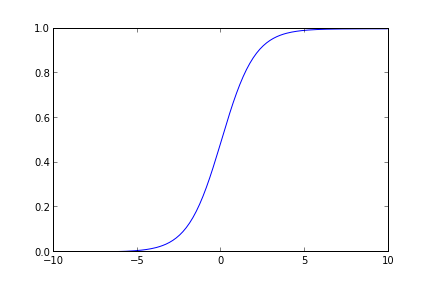
\includegraphics[height=6cm]{logreg1.png}

Altta veriyi işletmeden önce kendimiz karıştırıyoruz,

\begin{minted}[fontsize=\footnotesize]{python}
!sort --random-sort testSet.txt > /tmp/testSet1.txt
\end{minted}

\inputminted[fontsize=\footnotesize]{python}{logreg.py}

Üstte eşleyici içinde tek bir tane anahtar üretiyoruz, tüm makinalarda tüm
eşleyiciler aynı anahtarı, bir kez üretiyor olacaklar. Bunun sebebi nedir?
Ne yapmaya çalıştığımızı hatırlayalım, tüm makinalarda lojistik regresyon
işletiyoruz, gradyan çıkışı yapıyoruz, ve sonuçta o makinanın işi bitince
elimizde tek bir tane ağırlık vektörü yani theta olacak. İlgilendiğimiz
sonuç bu, o yüzden çıktı stdout'a tek bir satır yazılıyor. Peki niye aynı
anahtar? Çünkü her makinadaki tüm ağırlık vektörlerinin "hep beraber" bir
noktada ortalamasının alınmasını istiyoruz, bunu Hadoop'a yaptırmanın bir
yolu herkese aynı anahtarı kullandırtmak, böylece bu anahtarlar tek bir
indirgeyiciye (ve makinaya) gidecek, ve orada ortalamaları alınacak. Tüm
eşleyicilerin sonucunun tek bir indirgeçiye gitmesi performans problemi
çıkartmaz mı? Çıkmaz, çünkü 1000 tane, 10000 tane eşleyici paralel iş
yapmış olabilir, ama işleri bitince elimizde 1000,10000 tane ağırlık
vektörü olacak, ve bu zaten tek makinanın rahatlıkla başa çıkabileceği bir
yüktür.

Bu yaklaşım, eşleyicinin her veri satırı başına bir ya da daha fazla
anahtar-değer satırı ürettiği yaklaşımdan (mesela klasik kelime sayma
problemi) biraz farklı, o sebeple bu farklılığı belirtmek istedik.

Bir püf nokta, her veri satırı için işletilen map'e de aslında anahtar
ürettirmiyoruz, tüm map çağrıları bittikten sonra son bir kez çağırılacak
map\_final'a bu işi yaptırıyoruz. Oraya gelinceye kadar (map içinde) değişen
theta'yı sürekli hafızada tutmuşuz, son noktaya gelince o sonucu aynı
anahtar ile eşleyerek üretiyoruz ve iş bitiyor.

Komut satırından işletelim:

\begin{minted}[fontsize=\footnotesize]{python}
!python logreg.py /tmp/testSet1.txt 
\end{minted}

\begin{verbatim}
using configs in /home/burak/.mrjob.conf
creating tmp directory /tmp/logreg.burak.20131201.234703.391390
writing to /tmp/logreg.burak.20131201.234703.391390/step-0-mapper_part-00000
Counters from step 1:
  (no counters found)
writing to /tmp/logreg.burak.20131201.234703.391390/step-0-mapper-sorted
> sort /tmp/logreg.burak.20131201.234703.391390/step-0-mapper_part-00000
writing to /tmp/logreg.burak.20131201.234703.391390/step-0-reducer_part-00000
Counters from step 1:
  (no counters found)
Moving /tmp/logreg.burak.20131201.234703.391390/step-0-reducer_part-00000 -> /tmp/logreg.burak.20131201.234703.391390/output/part-00000
Streaming final output from /tmp/logreg.burak.20131201.234703.391390/output
"result"	"[[ 9.50705297]\n [-0.32580375]\n [-0.31237616]]"
removing tmp directory /tmp/logreg.burak.20131201.234703.391390
\end{verbatim}

\begin{minted}[fontsize=\footnotesize]{python}
def plot_theta(theta):
    x = np.array(arange(-10.0, 40.0, 0.1))
    y = np.array((-theta[0]-theta[1]*x)/theta[2])
    plot(x, y)
    hold(True)
    plot(d1.ix[:,0],d1.ix[:,1],'b.')
    hold(True)
    plot(d2.ix[:,0],d2.ix[:,1],'r.')
    hold(True)
    ylim(0,30)
    xlim(0,30)

theta = [9.50829527,-0.36317422,-0.34354905]
plot_theta(theta)
plt.savefig('logreg2.png')
\end{minted}

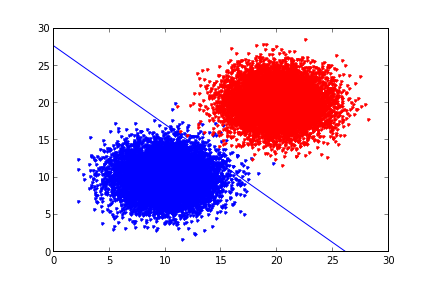
\includegraphics[height=5cm]{logreg2.png}

Kaynaklar

[1] Smola, {\em Scalable Machine Learning, Optimization}, \url{http://alex.smola.org/teaching/berkeley2012/slides/4_Optimization.pdf}

[2] Bhandarkar, {\em Modeling with Hadoop}, \url{http://www.slideshare.net/hadoop/modeling-with-hadoop-kdd2011}

[3] Simianer, {\em Joint Feature Selection in Distributed Stochastic Learning for Large-Scale Discriminative SMT}, \url{http://simianer.de/P12-1002-slides.pdf}

[4] Allen, {\em A Python implementation of binary regularized logistic
  regression with stochastic gradient descent, packaged as scripts for use
  with Hadoop streaming}, \url{https://github.com/elsevierlabs/logistic-regression-sgd-mapreduce}

\end{document}
